\newpage
\section{Diagrammi dei packages e delle classi}

\subsection{Introduzione}
Questa sezione racchiude i diagrammi dei packages, raccolti tramite un approccio top-down. \textbf{N.B.: raggiunto il sub-package minimo, si procederà con la descrizione delle classi implementate al suo interno}.\\Considerando l'approccio adottato e il particolare applicativo realizzato con un pattern a microservizi, il team non si discosterà dalla nomenclatura tradizionale di \textit{Classe}, intesa come una categoria di entità in grado di svolgere uno specifico compito. Per mantenere una conformità con lo standard UML, dunque, verrà utilizzato il termine \textit{classe} per indicare ciò che all'atto pratico sarà implementato come un microservizio vero e proprio, stand-alone, con i propri metodi, in grado di fornire la funzionalità preposta. Trattandosi di una progettazione con un livello di dettaglio intermedio, le classi non verranno definite, bensì verrà data una descrizione della loro funzionalità, lo scopo e le relazioni che intercorrono con le altre classi. Tale descrizione sarà integrata nella seguente descrizione dei packages al livello più basso dell'elenco.

L'applicativo API Market è strutturato, come di consueto, in un lato front-end ed un lato back-end, come mostrato dal diagramma seguente:

\begin{figure}[H]
	\centering
	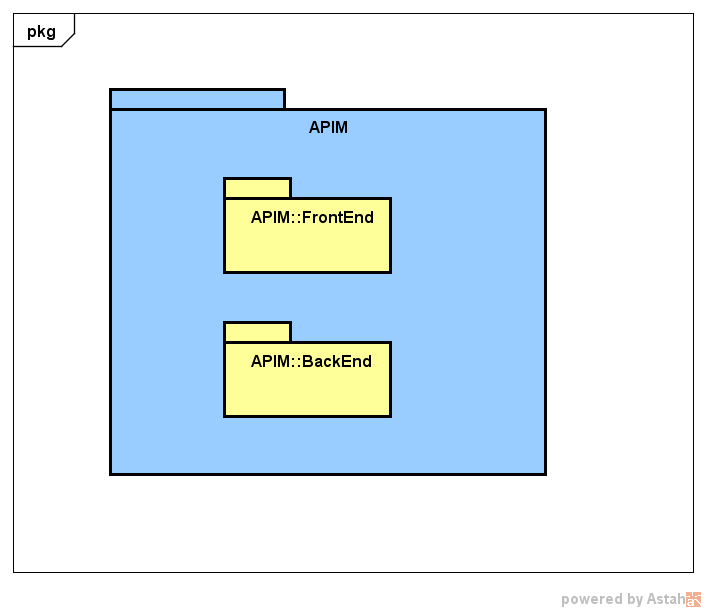
\includegraphics
	[width=0.7\linewidth]
	{UML/DiagrammiPackage/APIM.png}
	\caption{Package APIM}
\end{figure}

\newpage
\subsection{Front-end}

Il lato front-end risulta così strutturato:

\begin{figure}[H]
	\centering
	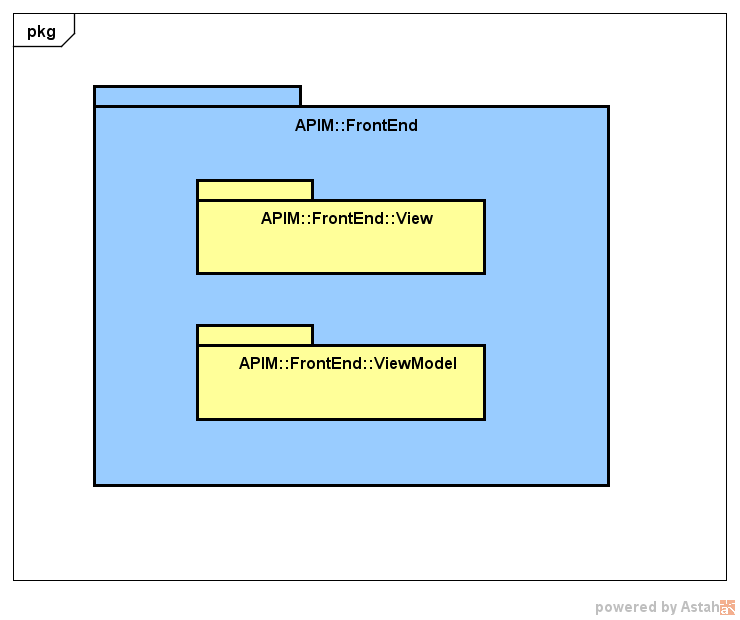
\includegraphics
	[width=0.7\linewidth]
	{UML/DiagrammiPackage/FrontEnd.png}
	\caption{Package APIM::FrontEnd}
\end{figure}

Nella parte front-end sono, dunque, presenti i package View e ViewModel, che rispecchiano l'architettura nativa dei framework scelti.

\begin{minipage}{\linewidth}
\subsubsection{View}

Il package per la componente View contiene i seguenti sub-packages:

\begin{figure}[H]
	\centering
	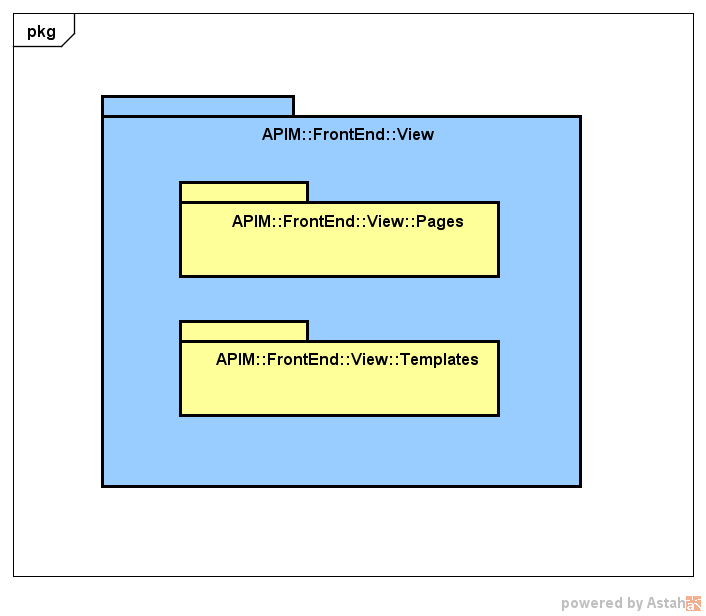
\includegraphics
	[width=0.7\linewidth]
	{UML/DiagrammiPackage/View.png}
	\caption{Package APIM::FrontEnd::View}
\end{figure}

\begin{itemize}
	\item \textbf{Pages}: il package \textit{Pages} contiene una classe astratta \textit{Page}. Essa è utilizzabile tramite una derivazione concreta di tale classe, e l'implementazione avviene a seconda di ciò che è necessario visualizzare. Tali implementazioni possono usufruire dei template, per gestire situazioni standardizzate.
	\item \textbf{Templates}: il package \textit{Templates} contiene un modello standard delle componenti utilizzabili per la rappresentazione. Ogni pagina che presenta situazioni e modelli analoghi può utilizzare un template già definito, per un maggior riuso, e per distinguere nettamente gli elementi contenuti in una pagina dalla loro realizzazione.
\end{itemize}
\end{minipage}

\paragraph{Pages}

\begin{figure}[H]
	\centering
	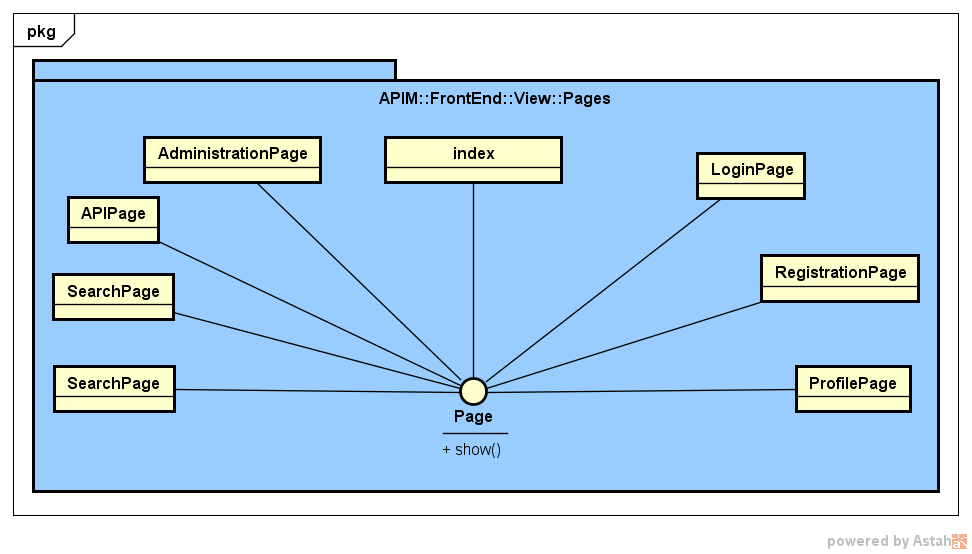
\includegraphics
	[width=0.7\linewidth]
	{UML/DiagrammiPackage/Pages.png}
	\caption{Package APIM::FrontEnd::View::Pages}
\end{figure}

\subparagraph{Page}
\begin{itemize}
	\item \textbf{Funzione del componente}: rappresenta una pagina web;
	\item \textbf{Relazioni d’uso di altri componenti}: interfaccia di base da cui derivano le altre pagine web;
	\item \textbf{Attività svolte e dati trattati}: definisce le caratteristiche minime che ogni pagina deve possedere.
\end{itemize}

\subparagraph{Index}
\begin{itemize}
	\item \textbf{Funzione del componente}: rappresenta la pagina principale dell'API Market;
	\item \textbf{Relazioni d’uso di altri componenti}: concretizza l'interfaccia \textit{Page} e utilizza i template \textit{MainMenu} e \textit{SearchForm};
	\item \textbf{Attività svolte e dati trattati}: permette l'autenticazione dell'utente e permette a un utente non autenticato di consultare una lista di API.
\end{itemize}

\subparagraph{LoginPage}
\begin{itemize}
	\item \textbf{Funzione del componente}: rappresenta la pagina di login;
	\item \textbf{Relazioni d’uso di altri componenti}: concretizza l'interfaccia \textit{Page} e utilizza i template \textit{MainMenu}, \textit{LoginForm}, \textit{PasswordRecoveryForm};
	\item \textbf{Attività svolte e dati trattati}: permette l'autenticazione dell'utente o il recupero della sua password.
\end{itemize}

\subparagraph{RegistrationPage}
\begin{itemize}
	\item \textbf{Funzione del componente}: rappresenta la pagina di registrazione;
	\item \textbf{Relazioni d’uso di altri componenti}: concretizza l'interfaccia \textit{Page} e utilizza il template \textit{MainMenu}, \textit{RegistrationForm};
	\item \textbf{Attività svolte e dati trattati}: permette la registrazione di un utente.
\end{itemize}

\subparagraph{ProfilePage}
\begin{itemize}
	\item \textbf{Funzione del componente}: rappresenta la pagina dove sono presenti le informazioni del profilo di un utente;
	\item \textbf{Relazioni d’uso di altri componenti}: concretizza l'interfaccia \textit{Page} e utilizza i template \textit{MainMenu}, \textit{ProfileForm}, \textit{EditProfileForm}, \textit{UserMenu}, \textit{TransactionList}, \textit{Transaction}, \textit{MyAPIList};
	\item \textbf{Attività svolte e dati trattati}: permette la consultazione dei dati di profilo a un utente registrato, la modifica dei dati del profilo, la visualizzazione delle API acquistate o registrate come lista o in dettaglio.
\end{itemize}

\subparagraph{AdministrationPage}
\begin{itemize}
	\item \textbf{Funzione del componente}: rappresenta la pagina di un amministratore;
	\item \textbf{Relazioni d’uso di altri componenti}: concretizza l'interfaccia \textit{Page} e utilizza il template \textit{MainMenu}, \textit{TransactionList}, \textit{UserList}, \textit{User}, \textit{TransactionList}, \textit{Transaction}, \textit{SearchForm}, \textit{SearchResult};
	\item \textbf{Attività svolte e dati trattati}: permette ad un amministratore di moderare gli utenti, vedere una lista di utenti e di API con possibilità di rimuovere un utente o un'API, ed effettuare una ricerca su utenti o API, vedendone il risultato.
\end{itemize}

\subparagraph{APIPage}
\begin{itemize}
	\item \textbf{Funzione del componente}: rappresenta la pagina di un'API o di una lista di API;
	\item \textbf{Relazioni d’uso di altri componenti}: concretizza l'interfaccia \textit{Page} e utilizza i template \textit{MainMenu}, \textit{APIList}, \textit{API}, \textit{SearchResult}, \textit{MyAPIList}, \textit{APIRegistrationForm}, \textit{APIEditForm}, \textit{CheckoutForm}, \textit{SearchForm}, \textit{SearchResult};
	\item \textbf{Attività svolte e dati trattati}: permette a un utente di consultare i dati di un'API, di ricercare un'API e vederne il risultato a schermo, consultare un lista di proprie API acquistate o registrate, e se le API sono proprie registrate, consente di modificarle. \MakeUppercase{è} possibile acquistare un'API e portare a termine l'acquisto tramite un form apposito.
\end{itemize}

\subparagraph{SearchPage}
\begin{itemize}
	\item \textbf{Funzione del componente}: rappresenta la pagina di ricerca;
	\item \textbf{Relazioni d’uso di altri componenti}: concretizza l'interfaccia \textit{Page} e utilizza i template \textit{MainMenu}, \textit{SearchForm} e \textit{SearchResult};
	\item \textbf{Attività svolte e dati trattati}: permette la ricerca di un'API o di un utente.	
\end{itemize}

\subparagraph{CategoryListPage}
\begin{itemize}
	\item \textbf{Funzione del componente}: rappresenta la pagina di una categoria;
	\item \textbf{Relazioni d’uso di altri componenti}: concretizza l'interfaccia \textit{Page} e utilizza i template \textit{MainMenu}, \textit{CategoryList} e \textit{Category};
	\item \textbf{Attività svolte e dati trattati}: permette la consultazione di un'API per categoria.
\end{itemize}


\paragraph{Templates}

\begin{figure}[H]
	\centering
	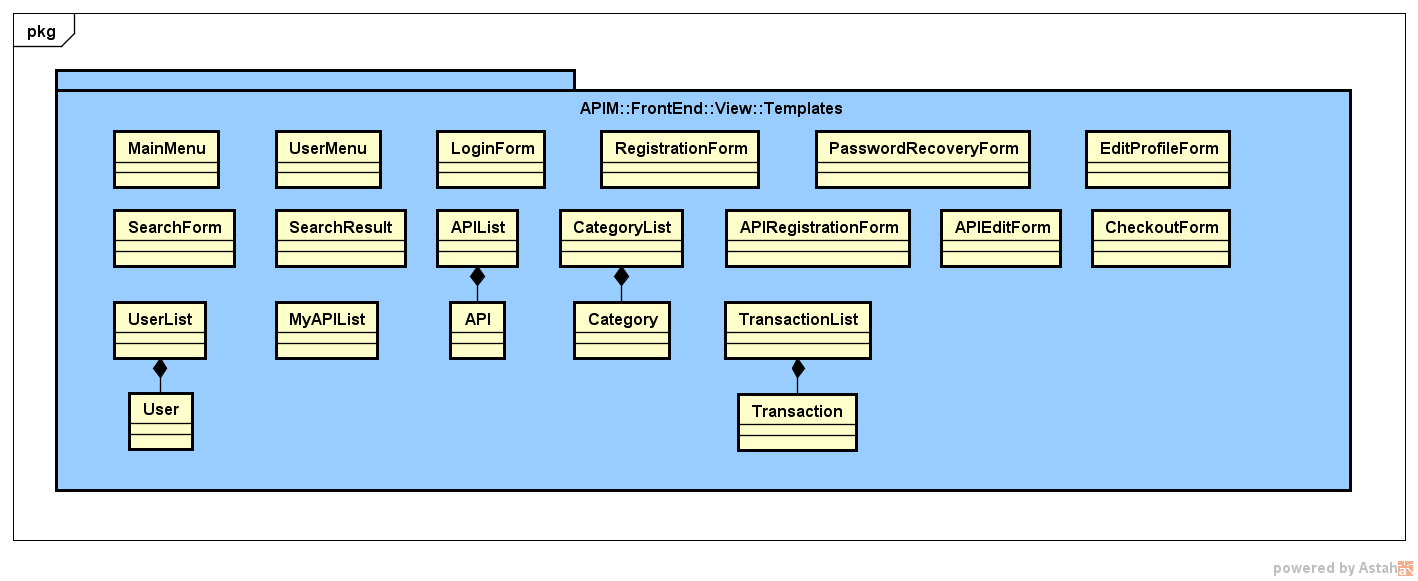
\includegraphics
	[width=0.7\linewidth]
	{UML/DiagrammiPackage/Templates.png}
	\caption{Package APIM::FrontEnd::View::Templates}
\end{figure}

\subparagraph{MainMenu}
\begin{itemize}
	\item \textbf{Funzione del componente}: rappresenta il template del menu principale;
	\item \textbf{Relazioni d’uso di altri componenti}: tutte le pagine derivate da \textit{Page};
	\item \textbf{Attività svolte e dati trattati}: è lo scheletro del menu che sarà presente su ogni pagina. Una sua modifica si rifletterà su tutte le view.
\end{itemize}

\subparagraph{UserMenu}
\begin{itemize}
	\item \textbf{Funzione del componente}: rappresenta il template del menu utente;
	\item \textbf{Relazioni d’uso di altri componenti}: tutte le pagine derivate da \textit{Page} di un utente autenticato;
	\item \textbf{Attività svolte e dati trattati}: è lo scheletro del menu utente.
\end{itemize}

\subparagraph{LoginForm}
\begin{itemize}
	\item \textbf{Funzione del componente}: rappresenta il template del form per il login;
	\item \textbf{Relazioni d’uso di altri componenti}: \textit{LoginPage};
	\item \textbf{Attività svolte e dati trattati}: è lo scheletro del form che sarà usato per autenticarsi all'applicazione web.
\end{itemize}

\subparagraph{RegistrationForm}
\begin{itemize}
	\item \textbf{Funzione del componente}: rappresenta il template del form per la registrazione;
	\item \textbf{Relazioni d’uso di altri componenti}: \textit{RegistrationPage};
	\item \textbf{Attività svolte e dati trattati}: è lo scheletro del form che sarà usato per registrarsi all'applicazione web.
\end{itemize}

\subparagraph{PasswordRecoveryForm}
\begin{itemize}
	\item \textbf{Funzione del componente}: rappresenta il template del form per il recupero della password;
	\item \textbf{Relazioni d’uso di altri componenti}: \textit{LoginPage};
	\item \textbf{Attività svolte e dati trattati}: è lo scheletro del form che sarà usato per recuperare la password.
\end{itemize}

\subparagraph{EditProfileForm}
\begin{itemize}
	\item \textbf{Funzione del componente}: rappresenta il template del form per la modifica del profilo utente;
	\item \textbf{Relazioni d’uso di altri componenti}: \textit{ProfilePage};
	\item \textbf{Attività svolte e dati trattati}: è lo scheletro del form che sarà usato per modificare il profilo.
\end{itemize}

\subparagraph{SearchForm}
\begin{itemize}
	\item \textbf{Funzione del componente}: rappresenta il template del form per la ricerca;
	\item \textbf{Relazioni d’uso di altri componenti}: \textit{SearchPage};
	\item \textbf{Attività svolte e dati trattati}: è lo scheletro del form che sarà usato per la ricerca.
\end{itemize}

\subparagraph{SearchResultForm}
\begin{itemize}
	\item \textbf{Funzione del componente}: rappresenta il template del form per visualizzare i risultati della ricerca;
	\item \textbf{Relazioni d’uso di altri componenti}: \textit{SearchPage};
	\item \textbf{Attività svolte e dati trattati}: è lo scheletro del form che sarà usato per visualizzare i risultati della ricerca.
\end{itemize}

\subparagraph{API}
\begin{itemize}
	\item \textbf{Funzione del componente}:  rappresenta il template della view usata per visualizzare i dati di un'API;
	\item \textbf{Relazioni d’uso di altri componenti}: \textit{APIPage};
	\item \textbf{Attività svolte e dati trattati}: è lo scheletro della view che sarà usata per visualizzare i dati di un'API.
\end{itemize}

\subparagraph{APIList}
\begin{itemize}
	\item \textbf{Funzione del componente}: rappresenta il template della view usata per visualizzare una lista di API;
	\item \textbf{Relazioni d’uso di altri componenti}: \textit{APIPage};
	\item \textbf{Attività svolte e dati trattati}: è lo scheletro della view che sarà usata per visualizzare una lista di API.
\end{itemize}

\subparagraph{Category}
\begin{itemize}
	\item \textbf{Funzione del componente}: rappresenta il template di una categoria;
	\item \textbf{Relazioni d’uso di altri componenti}: \textit{CategoryListPage};
	\item \textbf{Attività svolte e dati trattati}: \`{e} lo scheletro della view che sar\`{a} usata per visualizzare una categoria.
\end{itemize}

\subparagraph{CategoryList}
\begin{itemize}
	\item \textbf{Funzione del componente}: rappresenta il template della view che sar\`{a} usata per visualizzare una lista di categorie;
	\item \textbf{Relazioni d’uso di altri componenti}: \textit{CategoryListPage};
	\item \textbf{Attività svolte e dati trattati}: \`{e} lo scheletro della view che sar\`{a} usata per visualizzare una lista di categorie.
\end{itemize}

\subparagraph{APIRegistrationForm}
\begin{itemize}
	\item \textbf{Funzione del componente}: rappresenta il template del form per la registrazione di un'API;
	\item \textbf{Relazioni d’uso di altri componenti}: \textit{RegistrationPage};
	\item \textbf{Attività svolte e dati trattati}: \`{e} lo scheletro del form che sar\`{a} usato per la registrazione di un'API.
\end{itemize}

\subparagraph{APIEditForm}
\begin{itemize}
	\item \textbf{Funzione del componente}: rappresenta il template del form per modificare un'API;
	\item \textbf{Relazioni d’uso di altri componenti}: \textit{APIPage};
	\item \textbf{Attività svolte e dati trattati}: \`{e} lo scheletro del form che sar\`{a} usato per la modifica di un'API.
\end{itemize}

\subparagraph{CheckoutForm}
\begin{itemize}
	\item \textbf{Funzione del componente}: rappresenta il template del form per effettuare il checkout per l'acquisto un'API;
	\item \textbf{Relazioni d’uso di altri componenti}: \textit{APIPage};
	\item \textbf{Attività svolte e dati trattati}: \`{e} lo scheletro del form che sar\`{a} usato per effettuare il checkout per l'acquisto un'API.
\end{itemize}

\subparagraph{User}
\begin{itemize}
	\item \textbf{Funzione del componente}: rappresenta il template di un utente;
	\item \textbf{Relazioni d’uso di altri componenti}: \textit{AdministrationPage};
	\item \textbf{Attività svolte e dati trattati}: \`{e} lo scheletro della view che sar\`{a} usata per visualizzare un utente o i suoi dati.
\end{itemize}

\subparagraph{UserList}
\begin{itemize}
	\item \textbf{Funzione del componente}: rappresenta il template di una lista di utenti;
	\item \textbf{Relazioni d’uso di altri componenti}: \textit{AdministrationPage};
	\item \textbf{Attività svolte e dati trattati}: \`{e} lo scheletro della view che sar\`{a} usata per visualizzare una lista di utenti e i dati a loro pertinenti.
\end{itemize}

\subparagraph{MyAPIList}
\begin{itemize}
	\item \textbf{Funzione del componente}: rappresenta il template di una lista di API;
	\item \textbf{Relazioni d’uso di altri componenti}: \textit{APIPage}, \textit{ProfilePage};
	\item \textbf{Attività svolte e dati trattati}: \`{e} lo scheletro della view che sar\`{a} usata per visualizzare una lista di API e i dati a loro pertinenti.
\end{itemize}

\subparagraph{Transaction}
\begin{itemize}
	\item \textbf{Funzione del componente}: rappresenta il template di una transazione;
	\item \textbf{Relazioni d’uso di altri componenti}: \textit{ProfilePage}, \textit{AdministrationPage};
	\item \textbf{Attività svolte e dati trattati}: \`{e} lo scheletro della view che sar\`{a} usata per visualizzare una transazione e i dati a essa pertinenti.
\end{itemize}

\subparagraph{TransactionList}
\begin{itemize}
	\item \textbf{Funzione del componente}: rappresenta il template di una lista di transazioni;
	\item \textbf{Relazioni d’uso di altri componenti}: \textit{ProfilePage}, \textit{AdministrationPage};
	\item \textbf{Attività svolte e dati trattati}: \`{e} lo scheletro della view che sar\`{a} usata per visualizzare una lista di transazioni e i dati a loro pertinenti.
\end{itemize}

\begin{minipage}{\linewidth}
\subsubsection{ViewModel}

Il package per la componente ViewModel contiene i seguenti sub-packages:

\begin{figure}[H]
	\centering
	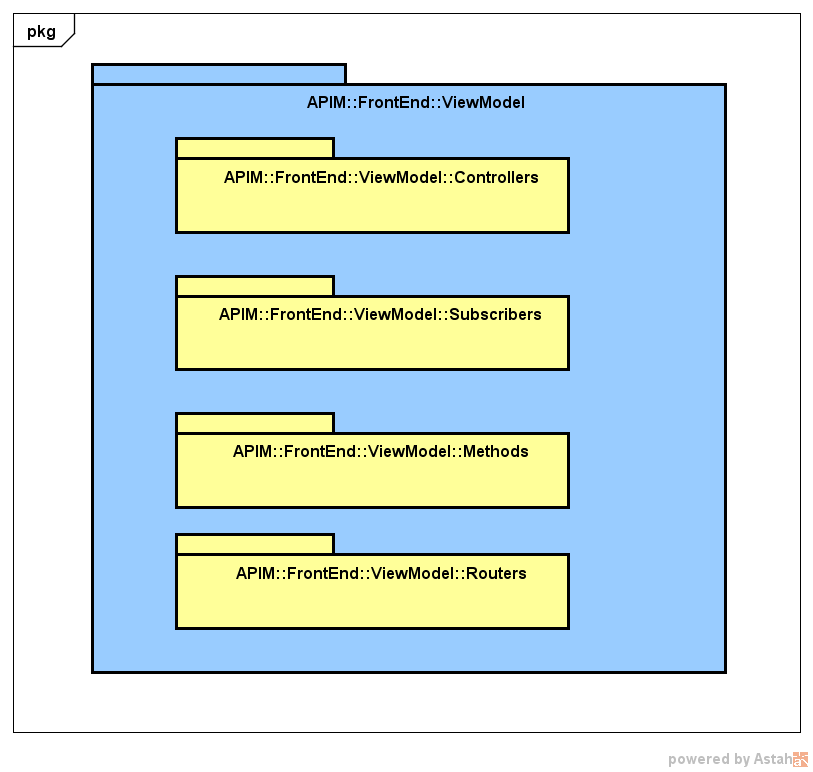
\includegraphics
	[width=0.7\linewidth]
	{UML/DiagrammiPackage/ViewModel.png}
	\caption{Package APIM::FrontEnd::ViewModel}
\end{figure}

La componente \textit{ViewModel} ha il compito di realizzare il data-binding con i componenti della \textit{View}, interagendo con la componente \textit{Model}, la quale fornisce i dati e ne permette la modifica. La componente \textit{Model} è parte del lato back-end della piattaforma, sebbene adottando un tale approccio si ha una linea di demarcazione meno netta tra le due parti. Di seguito, si analizzano i packages contenuti all'interno del componente \textit{ViewModel}:

\begin{itemize}
	\item \textbf{Controllers}: contiene i controller necessari alle views per comunicare con il \textit{Model};
	\item \textbf{Subscribers}: contiene le classi necessarie al subscribing alle collezioni pubblicate dai \textit{Publisher};
	\item \textbf{Methods}: contiene le classi necessarie a MeteorJS per la corretta fruizione dei dati;
	\item \textbf{Routers}: contiene la classe che esegue il routing dell'intera applicazione. 
\end{itemize}
\end{minipage}

\paragraph{Controllers}

\begin{figure}[H]
	\centering
	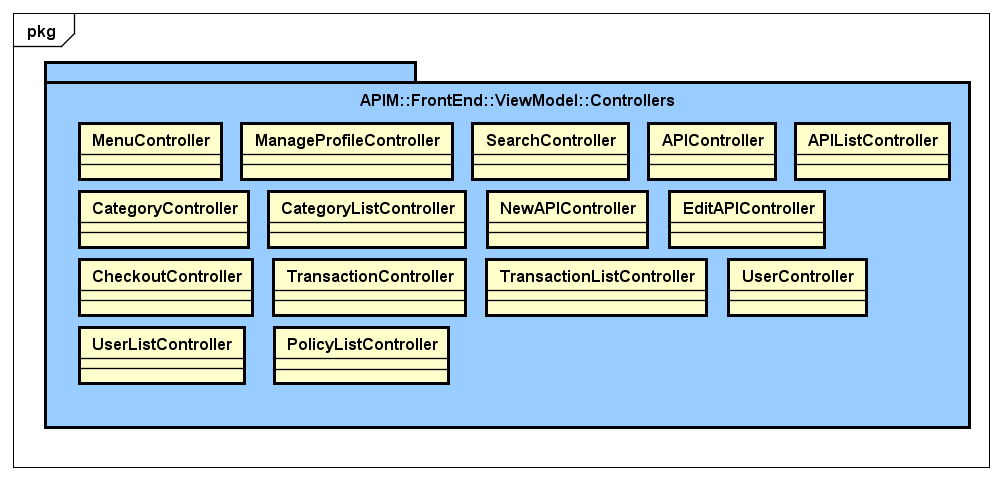
\includegraphics
	[width=0.7\linewidth]
	{UML/DiagrammiPackage/Controllers.png}
	\caption{Package APIM::FrontEnd::ViewModel::Controllers}
\end{figure}

\subparagraph{MenuController}
\begin{itemize}
	\item \textbf{Funzione del componente}: la classe permette la corretta visualizzazione del menu, in base ai propri privilegi;
	\item \textbf{Relazioni d’uso di altri componenti}: il controller è collegato ai template \textit{MainMenu} e \textit{UserMenu}.
\end{itemize}

\subparagraph{ManageProfileController}
\begin{itemize}
	\item \textbf{Funzione del componente}: permette la gestione del proprio profilo utente;
	\item \textbf{Relazioni d’uso di altri componenti}: utilizza i template \textit{TransactionList}, \textit{Transaction}, \textit{EditProfileForm}, \textit{MyAPIList};
	\item \textbf{Attività svolte e dati trattati}: coordina tutte le funzionalità di gestione che può svolgere un utente registrato, come gestire le proprie transazioni e vedere lo stato dei suoi abbonamenti. 
\end{itemize}

\subparagraph{SearchController}
\begin{itemize}
	\item \textbf{Funzione del componente}: permette la gestione della ricerca;
	\item \textbf{Relazioni d’uso di altri componenti}: utilizza i template \textit{SearchForm}, \textit{SearchResult};
	\item \textbf{Attività svolte e dati trattati}: coordina tutte le funzionalità di ricerca che può svolgere un utente non registrato o registrato, in base ai privilegi annessi.
\end{itemize}

\subparagraph{APIController}
\begin{itemize}
	\item \textbf{Funzione del componente}: permette la gestione di un'API;
	\item \textbf{Relazioni d’uso di altri componenti}: utilizza i templates \textit{TransactionList}, \textit{Transaction}, \textit{EditProfileForm}, \textit{MyAPIList};
	\item \textbf{Attività svolte e dati trattati}: coordina tutte le funzionalità di visualizzazione e interazione con un'API.
\end{itemize}

\subparagraph{APIListController}
\begin{itemize}
	\item \textbf{Funzione del componente}: permette la gestione di una lista di API;
	\item \textbf{Relazioni d’uso di altri componenti}: 
	\item \textbf{Attività svolte e dati trattati}: coordina tutte le funzionalità di visualizzazione e interazione con una lista di API.
\end{itemize}

\subparagraph{CategoryController}
\begin{itemize}
	\item \textbf{Funzione del componente}: permette la gestione di una categoria;
	\item \textbf{Relazioni d’uso di altri componenti}: utilizza il template \textit{Category};
	\item \textbf{Attività svolte e dati trattati}: coordina tutte le funzionalità di visualizzazione e interazione con una categoria.
\end{itemize}

\subparagraph{CategoryListController}
\begin{itemize}
	\item \textbf{Funzione del componente}: permette la gestione di una lista di categorie;
	\item \textbf{Relazioni d’uso di altri componenti}: utilizza il template \textit{CategoryList};
	\item \textbf{Attività svolte e dati trattati}: coordina tutte le funzionalità di visualizzazione e interazione con una lista di categorie.
\end{itemize}

\subparagraph{NewAPIController}
\begin{itemize}
	\item \textbf{Funzione del componente}: permette la creazione di un'API;
	\item \textbf{Relazioni d’uso di altri componenti}: utilizza il template \textit{APIRegistrationForm};
	\item \textbf{Attività svolte e dati trattati}: coordina tutte le funzionalità di visualizzazione e interazione nel contesto dell'inserimento di una nuova API.
\end{itemize}

\subparagraph{EditAPIController}
\begin{itemize}
	\item \textbf{Funzione del componente}: permette la modifica di un'API;
	\item \textbf{Relazioni d’uso di altri componenti}: utilizza il template \textit{APIEditForm};
	\item \textbf{Attività svolte e dati trattati}: coordina tutte le funzionalità di visualizzazione e interazione nel contesto della modifica di un'API.
\end{itemize}

\subparagraph{CheckoutController}
\begin{itemize}
	\item \textbf{Funzione del componente}: permette il checkout;
	\item \textbf{Relazioni d’uso di altri componenti}: utilizza il template \textit{CheckoutForm};
	\item \textbf{Attività svolte e dati trattati}: coordina tutte le funzionalità di visualizzazione e interazione nel contesto del checkout per l'acquisto di un'API.
\end{itemize}

\subparagraph{TransactionController}
\begin{itemize}
	\item \textbf{Funzione del componente}: permette la gestione di una transazione;
	\item \textbf{Relazioni d’uso di altri componenti}: utilizza il template \textit{Transaction};
	\item \textbf{Attività svolte e dati trattati}: coordina tutte le funzionalità di visualizzazione e interazione con una transazione.
\end{itemize}

\subparagraph{TransactionListController}
\begin{itemize}
	\item \textbf{Funzione del componente}: permette la gestione di una lista di transazioni;
	\item \textbf{Relazioni d’uso di altri componenti}: utilizza il template \textit{TransactionList};
	\item \textbf{Attività svolte e dati trattati}: coordina tutte le funzionalità di visualizzazione e interazione con una lista di transazioni.
\end{itemize}

\subparagraph{UserController}
\begin{itemize}
	\item \textbf{Funzione del componente}: permette la gestione di un utente;
	\item \textbf{Relazioni d’uso di altri componenti}: utilizza il template \textit{User};
	\item \textbf{Attività svolte e dati trattati}: coordina tutte le funzionalità di visualizzazione e interazione con un utente.
\end{itemize}

\subparagraph{UserListController}
\begin{itemize}
	\item \textbf{Funzione del componente}: permette la gestione di una lista di utenti;
	\item \textbf{Relazioni d’uso di altri componenti}: utilizza il template \textit{UserList};
	\item \textbf{Attività svolte e dati trattati}: coordina tutte le funzionalità di visualizzazione e interazione con una lista di utenti.
\end{itemize}

\subparagraph{PolicyListController}
\begin{itemize}
	\item \textbf{Funzione del componente}: permette la gestione di una lista di policy;
	\item \textbf{Attività svolte e dati trattati}: coordina tutte le funzionalità di visualizzazione e interazione con una lista di policy.
\end{itemize}


\paragraph{Subscribers}

\begin{figure}[H]
	\centering
	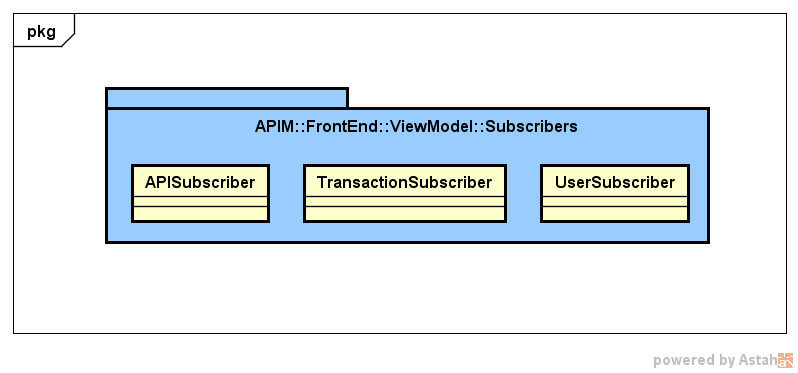
\includegraphics
	[width=0.7\linewidth]
	{UML/DiagrammiPackage/Subscribers.png}
	\caption{Package APIM::FrontEnd::ViewModel::Subscribers}
\end{figure}

\subparagraph{APISubscriber}
\begin{itemize}
	\item \textbf{Funzione del componente}: la classe esegue il subscribing delle API.
	\item \textbf{Relazioni d’uso di altri componenti}: è in relazione con l'\textit{APIController}.
	\item \textbf{Attività svolte e dati trattati}: esegue il subscribing di quelle collezioni di cui è stato precedentemente fatto il publishing.
\end{itemize}

\subparagraph{TransactionSubscriber}
\begin{itemize}
	\item \textbf{Funzione del componente}: la classe esegue il subscribing delle transazioni.
	\item \textbf{Relazioni d’uso di altri componenti}: è in relazione con il \textit{TransactionController}.
	\item \textbf{Attività svolte e dati trattati}: esegue il subscribing di quelle collezioni di cui è stato precedentemente fatto il publishing.
\end{itemize}

\subparagraph{UserSubscriber}
\begin{itemize}
	\item \textbf{Funzione del componente}: la classe esegue il subscribing degli utenti.
	\item \textbf{Relazioni d’uso di altri componenti}: è in relazione con lo \textit{UserController}.
	\item \textbf{Attività svolte e dati trattati}: esegue il subscribing di quelle collezioni di cui è stato precedentemente fatto il publishing.
\end{itemize}

\paragraph{Methods}

\begin{figure}[H]
	\centering
	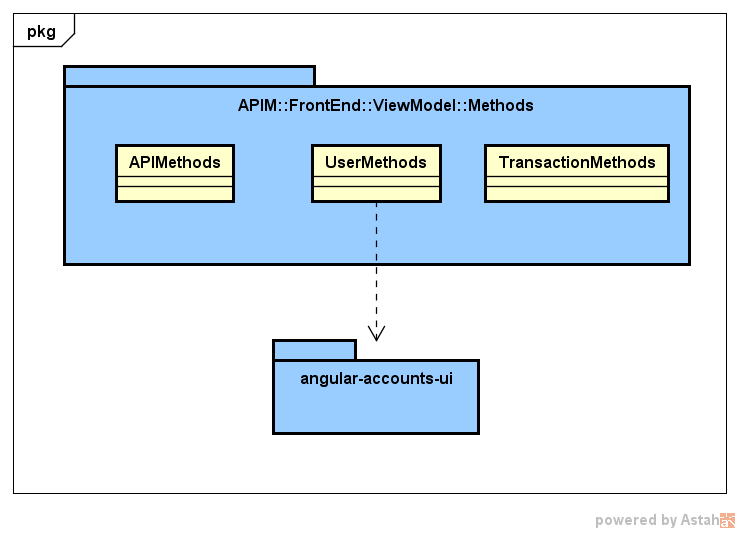
\includegraphics
	[width=0.7\linewidth]
	{UML/DiagrammiPackage/Methods.png}
	\caption{Package APIM::FrontEnd::ViewModel::Methods}
\end{figure}

\subparagraph{APIMethods}
\begin{itemize}
	\item \textbf{Funzione del componente}: la classe viene utilizzata dal front-end per richiedere una modifica delle API;
	\item \textbf{Relazioni d’uso di altri componenti}: è in relazione con \textit{NewAPIController} e \textit{EditAPIController};
	\item \textbf{Attività svolte e dati trattati}: fornisce all'utente le funzioni di inserimento, modifica e cancellazione delle API.
\end{itemize}

\subparagraph{TransactionMethods}
\begin{itemize}
	\item \textbf{Funzione del componente}: la classe viene utilizzata dal front-end per richiedere una modifica delle transazioni;
	\item \textbf{Relazioni d’uso di altri componenti}: è in relazione con \textit{NewTransactionController} e \textit{EditTransactionController};
	\item \textbf{Attività svolte e dati trattati}: fornisce all'utente le funzioni di inserimento, modifica e cancellazione delle transazioni.
\end{itemize}

\subparagraph{UserMethods}
\begin{itemize}
	\item \textbf{Funzione del componente}: la classe viene utilizzata dal front-end per richiedere una modifica degli utenti;
	\item \textbf{Relazioni d’uso di altri componenti}: è in relazione con il package esterno \textit{angular-accounts-ui};
	\item \textbf{Attività svolte e dati trattati}: fornisce all'utente le funzioni di inserimento, modifica e cancellazione degli utenti.
\end{itemize}


\paragraph{Routers}

\begin{figure}[H]
	\centering
	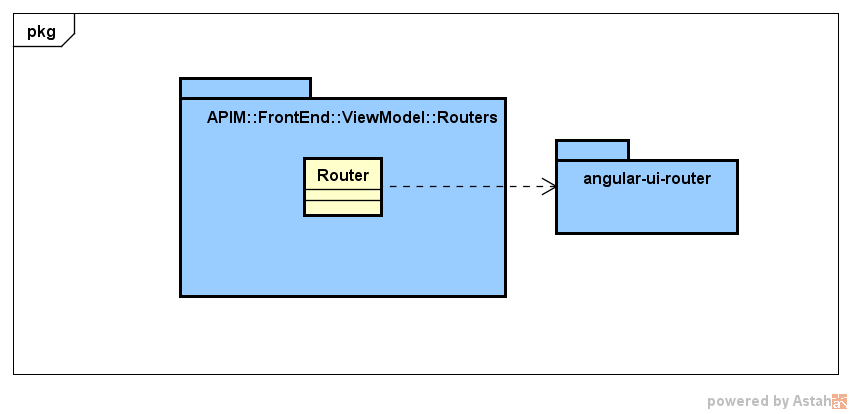
\includegraphics
	[width=0.7\linewidth]
	{UML/DiagrammiPackage/Routers.png}
	\caption{Package APIM::FrontEnd::ViewModel::Routers}
\end{figure}

\subparagraph{Router}
\begin{itemize}
	\item \textbf{Funzione del componente}: la classe permette il routing dinamico delle pagine;
	\item \textbf{Relazioni d’uso di altri componenti}: è in relazione con il package esterno \textit{angular-ui-router} e con tutte le pages e i templates;
	\item \textbf{Attività svolte e dati trattati}: esegue la traduzione degli URL in modo dinamico, permettendo la visualizzazione in modalità one-page, senza bisogno di ricaricare l'intera pagina.
\end{itemize}